\documentclass[12pt]{article}
\usepackage{lingmacros}
\usepackage{tree-dvips}
\usepackage{amsmath}
\usepackage{tabularx}
\usepackage{mathtools}
\usepackage{graphicx}
\graphicspath{ {./images/}}
\DeclarePairedDelimiter\ceil{\lceil}{\rceil}
\DeclarePairedDelimiter\floor{\lfloor}{\rfloor}

\begin{document}

\begin{titlepage}
    \begin{center}
        \vspace*{1cm}
         \textbf{\huge Artificial neural networks} \\        
        \vspace{0.30cm}
         {\LARGE Convolutional neural networks }\\
         \vspace{0.30cm}
         {\Large Traffic Sign Recognition }\\
        \vfill
        
        

        Adrián Vázquez Barrera \\
        \vspace{0.25cm}
        Polytechnic University of Valencia\\
        \vspace{0.25cm}
        \textbf{January 2022}
             
    \end{center}
 \end{titlepage}

\newpage

\section*{Contexto}
Se ha desarrollado una red neuronal convolucional especializada en reconocer 42 señales alemanas de tráfico. Para ello, se ha utilizado el conjunto de datos GTSRB alojado en la plataforma Kaggle.
Este dataset cuenta con más de 50 mil imágenes, con sub-conjuntos de entrenamiento y test previamente separados. Lo que es de agradecer, puesto que no encontramos el mismo número de ejemplos para todas las clases existentes y ahorra trabajo de preprocesamiento.
~\\\\
Adicionalmente, se ha enfocado el desarrollo de la práctica a una visión de producto, más que investigación. Es por ello que, además del estudio y análisis del estado del arte para esta tarea. Se ha implementado un contenedor Docker que lee un modelo pre-entrenado y automáticamente sirve de reconocedor de imágenes a través de un servidor web. Esto permitirá acoplar el modelo a cualquier aplicación existente con independencia de las tecnologías (o versiones existentes) empleadas.

\newpage

\section*{Diseño de la red}

La estructura de la red se fundamenta en la popular arquitectura VGG (Visual Geometry Group) que se basa en una sucesión profunda de capas convolucionales.
La arquitectura VGG es la base de modelos innovadores de reconocimiento de objetos, superando los límites establecidos en muchas tareas y conjuntos de datos más allá de ImageNet.
\\\\
\begin{center}
    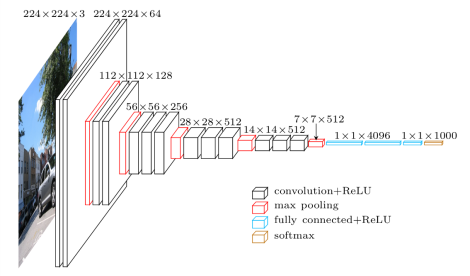
\includegraphics[scale=0.7]{vgg.png}
\end{center}
~\\
Solo con aplicar esta arquitectura no es suficiente para obtener una tasa de error de al rededor del 2\% que sería lo aceptable. Adicionalmente, se han implementado algoritmos de Mix-Up y Cut-Out. Este último es una función acoplada al Data-generator que, dada una imagen, elimina fragmentos de esta. Lo que obliga a la red a aprender exclusivamente aquellos elementos fundamentales de las muestras en el entrenamiento. Por otro lado, con Mix-Up conseguimos fusionar dos muestras del conjunto de entrenamiento para construir una nueva imagen modificando el canal alpha. Con ello, establecemos deliberadamente la preponderancia de una imagen sobre otra en un 10\%. Lo que añade ruido en el entrenamiento, evitando el sobre-aprendizaje de ciertos atributos y ayuda a mejorar la red cuando haya confusión entre dos clases. 

\newpage

\section*{Implementación de la red}

Tal y como se mencionó en el apartado anterior, la arquitectura de la red utilizada corresponda a una VGG. El número de epochs se ha establecido en 115 con un batch size de 1024. El factor de aprendizaje se encuentra originalmente establecido a 0.001, aunque durante el entrenamiento se hace uso de la técnica "Learning Rate Annealing" con el siguiente planificador:

\begin{equation*}
        scheduler(epoch) = learning\_rate \cdot 2^{- \floor*{ \frac{epoch}{20}}}
\end{equation*}
\\
Se ha apostado por el optimizador Adam, y los siguientes valores para el Data Augmentation:
\\\\
\begin{tabularx}{\textwidth} { 
    | >{\centering\arraybackslash}X 
    | >{\centering\arraybackslash}X |}
   \hline
   \multicolumn{2}{|c|}{Data Augmentation} \\
   \hline
   Rotation range & 10 degrees\\
  \hline
  Zoom range & 0.15 \\
  \hline
  Width shift range & 0.1 \\
  \hline
  Height shift range & 0.1 \\
  \hline
  Shear range & 0.15 \\
  \hline
  Horizontal flip & True \\
  \hline
  Vertical flip & False \\
  \hline
  Cut-Out & Area $\in (0, 1)$ \\
  \hline
  Mix-Up & 0.1 \\
  \hline
\end{tabularx}
\\\\\\
Al mismo tiempo, la red guardará una copia del modelo cuando exista un epoch que mejore la tasa de acierto con respecto al conjunto de test.
\\\\\\
\begin{tabularx}{\textwidth} { 
    | >{\centering\arraybackslash}X 
    | >{\centering\arraybackslash}X |}
   \hline
   \multicolumn{2}{|c|}{Experimentación} \\
  \hline
   4 capas convolucionales: CIFAR original de prácticas modificado. + Adam + Data Aug. & 96.3\%\\
  \hline
  Cambio de estructura a VGG + CutOut & 97.04 \%\\
  \hline
  Aumento y de atributos data augmentation, modificado Cut-Out + Mix-up  & 98.95 \%\\
  \hline
\end{tabularx}

\newpage

\section*{Despliegue de la red}
El desplieggue del sistema se ha llevado a cabo utilizando un contenedor docker a partir de una imagen vanilla de python 3.9.7, a la que se ha añadido TensorFlow 2.5.0, Numpy 1.19.5 y OpenCV. La aplicación además emplea las herramientas del lenguaje para habilitar un servidor HTTP que acepta peticiones POST.  
\\\\
Para realizar una predicción, será necesario enviar una petición web a la dirección IP de la máquina y adjuntar una imagen en formato PNG con la señal de tráfico a reconocer.   

\newpage

\section*{Bibliografía}
1. GTSRB - German Traffic Sign Recognition Benchmark - Multi-class, single-image classification challenge.
\\
https://www.kaggle.com/meowmeowmeowmeowmeow/gtsrb-german-traffic-sign
\\\\
2. VGG Very Deep Convolutional Networks (VGGNet) - What you need to know.
\\
https://viso.ai/deep-learning/vgg-very-deep-convolutional-networks
\\\\
3. MixUp augmentation for image classification.
\\
https://keras.io/examples/vision/mixup
\\\\
4. Cutout regularization for CNNs.
\\
https://medium.com/@ombelinelag/cutout-regularization-for-cnns-62670d86bc33

\end{document}

